% Figura Anexo I: la pendiente psi no es estructural: cae con la varianza de los precios que la propia política genera
\documentclass[tikz,border=3pt]{standalone}
\usepackage[T1]{fontenc}
\usepackage[utf8]{inputenc}
\usepackage{amsmath}
\usetikzlibrary{arrows.meta,calc,positioning}
\begin{document}
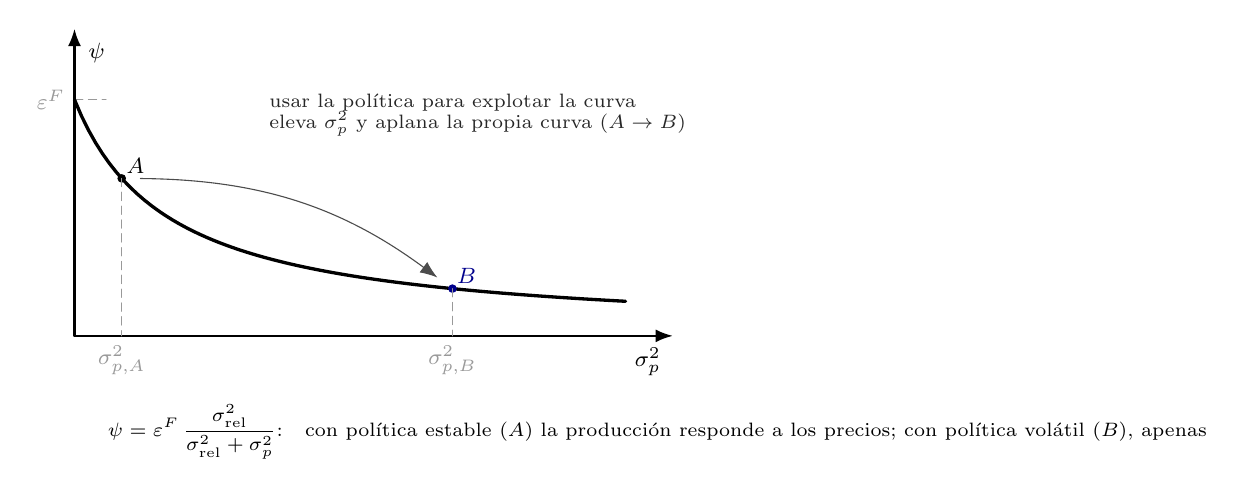
\begin{tikzpicture}[>={Latex[length=2.2mm]}, line cap=round, font=\footnotesize,
  eje/.style={->, thick},
  curva/.style={very thick},
  guia/.style={densely dashed, gray!80},
  pto/.style={circle, fill=black, inner sep=1.1pt}]
  \draw[eje] (0,0) -- (7.6,0) node[below left=1pt]{$\sigma^2_p$};
  \draw[eje] (0,0) -- (0,3.9) node[below right=2pt]{$\psi$};
  \draw[guia] (0,3.0) node[left]{$\varepsilon^F$} -- (0.4,3.0);
  \draw[curva, domain=0:7.0, samples=80] plot (\x,{3.0*1.2/(1.2+\x)});
  \node[pto] (A) at (0.6,2.0) {};
  \node[above right=-1pt of A, inner sep=1pt] {$A$};
  \node[pto, fill=blue!55!black] (B) at (4.8,0.6) {};
  \node[above right=-1pt of B, inner sep=1pt, blue!55!black] {$B$};
  \draw[guia] (0.6,2.0) -- (0.6,0) node[below]{$\sigma^2_{p,A}$};
  \draw[guia] (4.8,0.6) -- (4.8,0) node[below]{$\sigma^2_{p,B}$};
  \draw[->, gray!60!black, shorten >=5pt, shorten <=5pt] (A) to[bend left=18] (B);
  \node[align=left, anchor=west, gray!30!black] at (2.35,2.8) {\scriptsize usar la política para explotar la curva\\[-2pt]\scriptsize eleva $\sigma^2_p$ y aplana la propia curva ($A\to B$)};
  \node[align=left, anchor=north west] at (0.3,-0.75) {\scriptsize $\psi=\varepsilon^F\,\dfrac{\sigma^2_{\mathrm{rel}}}{\sigma^2_{\mathrm{rel}}+\sigma^2_p}$:\quad con política estable ($A$) la producción responde a los precios; con política volátil ($B$), apenas};
\end{tikzpicture}
\end{document}
